\section{Controlled empirical usability experiment}
\label{sec:experiment}

In November 2018, I conducted an experiment with students to evaluate some features of the Sensei \gls{ide} plugin.
This experiment has been well designed with the help of my supervisors and prof. Riccardo Scandariato who has practical experience with similar experiments.
It was conducted with the help of the lecturer, dr.\ Mattias De Wael, and two of my colleagues at \gls{scw}, Downey Robersscheuten and Tim Dekiere.

\subsection{Goals and research questions}
The main \textit{goal} of the experiment is to observe the impact of the Sensei \gls{ide} plugin on developers and developed code during development.
The \textit{purpose} is evaluating the usability and effectiveness of Sensei in supporting the paved path methodology.
The \textit{quality focus} is the ability of the plugin to help developers adhere to secure coding guidelines without causing a significant cognitive burden.
The study evaluates the behaviour of a developer.
We aim at measuring the increase in cognitive burden when developers use the plugin, by measuring the impact on development time.
In our experiment, we evaluated the impact on a group of students who have a consolidated minimum level of expertise in both web application development and web application security.

The above goal can be achieved by means of an experiment aimed at answering the following four questions:
\begin{itemize}
    \item \textbf{Q1} How effective are the Sensei code markings at grabbing the developer's attention?
    \item \textbf{Q2} Does the plugin significantly impact the development time?
    \item \textbf{Q3} Do developers often use the provided remediation (quick-fixes) to resolve code markings?
    \item \textbf{Q4} Are there any specific code markings that significantly impact the usability compared to others?
\end{itemize}

\subsection{Experimental set-up}
\subsubsection{Subjects}
The subjects for this study are a group of third year students following the bachelor program for Computer and Cyber Crime Professional\footnote{\url{https://www.howest.be/en/study-programmes?s_filter=bachelor}} at the college Hogeschool West-Vlaanderen (Howest) in Bruges, Belgium.
All students are in the third, and final year of the bachelor program.
The experiment was performed in the context of the Secure Object Oriented Architectures class.
In this course, the students are taught design patterns, how to design three-layered applications, and Java technicalities.
During the entire course the focus is on development while conforming to Oracle's Secure Coding Guidelines\footnote{\url{https://docs.oracle.com/cd/E26502\_01/html/E29016/scode-1.html}}.

All of the students are familiar with Java programming in IntelliJ IDEA, as it is the main language and \gls{ide} used in the education program.
They are, however, not experienced or trained with the Sensei tool.
This experiment was their first exposure to the tool. 

The experiment was preceded by a secure coding tournament using the \gls{scw} platform.
The goal of this tournament was to both engage the students as well as measure their skill level.
Student participation was voluntary, out of the 75 students that participated in the tournament, 60 also participated in the experiment itself.
However, only 32 students successfully submitted all necessary files after the experiment, as will be described further down this section.

\subsubsection{Development task}
\label{sec:task}
The subjects were given a development task to complete with the Sensei plugin installed in their \gls{ide}.
For the assignment they received the incomplete code for an employment web app.
The application provides employees of a company a way to view, download, and upload their payslips, as well as to submit requests for absence.
The application is written in Java and uses \gls{jsp} as the server side technology.
Some of the features are incomplete and must be completed by the subjects during the experiment.
During the implementation of these features, the subjects are at risk of introducing a number of web application vulnerabilities.
Below is a list of features to be completed and their associated risks.

\begin{itemize}[noitemsep]
    \item A web page to view absence requests: risk of \gls{xss}.
    \item A web form to search for absence requests in the database: risk of \gls{sql} injection.
    \item A web form to upload payslips in \gls{xml} format: risk of \gls{xml} injection, \gls{xml} external entity, unrestricted file upload, and local file inclusion.
    \item Log all attempts made on the sign-in page: risk of log forgery.
\end{itemize}

\subsubsection{Treatment}
The treatment consisted of two parts. First, all subjects participated in a \gls{scw} tournament.
The next week, all participants were given the Sensei \gls{ide} plugin, but some features were disabled for the control group.
\paragraph{Tournament}
One week preceding the experiment, all subjects participated in a tournament on the \gls{scw} platform.
The subjects were handed 24 secure coding exercises in Java using \gls{jsp} to complete within 90 minutes.
The awarded points on completion of an exercise depends on its difficulty and the performance of the subject, as described in Appendix~\ref{app:challenges}.
The scoring method chosen was ``Forgiving".

The total maximum score for all exercises in the tournament was 5000 points.
The highest score reached was 4920, while the lowest was 1600.
The mean score reached by the participants (n = 75) was 3659 (s = 710).
The mean time spent solving all exercises was 53.70 min (s = 16.07 min).
Both the score and the time spent are approximately normal distributions as shown in Figure~\ref{fig:hist-score} and Figure~\ref{fig:hist-time}.
The score reached by each subject in this tournament was used to split the subjects into two equally skilled groups, a control group and a test group.
The subjects were told that they were participating in an experiment regarding the Sensei plugin.
They were told that they were split in a control group and test group but were not informed of which group they were part, or what the difference in treatment would be. 

\begin{figure}
    \centering
    %\begin{tikzpicture}
    \node at (0,0) {
        \begin{tikzpicture}
        \begin{axis}[
            %ybar interval,
            ymax=24, ymin=0,
            xmin=1500, xmax=5000,
            xtick = {1500,5000},
            xtick pos=bottom,
            grid=none,
            ytick pos=left,
            ytick = {-1,25},
            y axis line style={draw=none},
            x axis line style={color=gray},
            x tick label style={color=gray,
                yshift={-1em},
                /pgf/number format/.cd,fixed,precision=3, set thousands separator={}},
            y tick label style={color=gray},
            ]
            
            \addplot [
            scw-teal,
            fill=scw-teal,
            ybar interval,
            mark=none,
            ]
            coordinates
            {
            (1500, 2)
            (2000, 1)
            (2500, 10)
            (3000, 14)
            (3500, 24)
            (4000, 14)
            (4500, 9)
            (5000, 0)
            };
    
        \end{axis}
        \end{tikzpicture}
    };
    
    %x axis
    \node[gray] at (0.9,-3.05) {3659 points};
    \draw[thick, lightgray] (-3.47,-2.7) -- (3.42,-2.7);
    \draw[thick, lightgray] (-3.47,-2.7) -- (-3.47,-2.6);
    \draw[thick, lightgray] (3.42,-2.7) -- (3.42,-2.6);
    \draw[thick, lightgray] (0.9,-2.7) -- (0.9,-2.6);
    
\end{tikzpicture}
  \includegraphics[page=17]{03-education/figures/tikzfigures.pdf}
  \caption[Histogram of points scored in the \gls{scw} tournament]{The points scored by the subjects during the tournament is approximately a normal distribution around the mean of 3659 points.}
  \label{fig:hist-score} 
\end{figure}

\begin{figure}
    \centering
  % \begin{tikzpicture}
    \node at (0,0) {
        \begin{tikzpicture}
        \begin{axis}[
            %ybar interval,
            ymax=17, ymin=0,
            xmin=10, xmax=100,
            xtick = {10,100},
            xtick pos=bottom,
            grid=none,
            ytick pos=left,
            ytick = {-1,20},
            y axis line style={draw=none},
            x axis line style={color=gray},
            x tick label style={color=gray, yshift={-1em}},
            y tick label style={color=gray},
            ]
            
            \addplot [
            scw-teal,
            fill=scw-teal,
            ybar interval,
            mark=none,
            ]
            coordinates
            {
            (10, 1)
            (20, 4)
            (30, 11)
            (40, 17)
            (50, 15)
            (60, 15)
            (70, 9)
            (80, 2)
            (90, 1)
            (100, 0)
            };
    
        \end{axis}
        \end{tikzpicture}
    };
    
    %x axis
    \node[gray] at (0,-3.05) {54 min};
    \draw[thick, lightgray] (-3.47,-2.7) -- (3.42,-2.7);
    \draw[thick, lightgray] (-3.47,-2.7) -- (-3.47,-2.6);
    \draw[thick, lightgray] (3.42,-2.7) -- (3.42,-2.6);
    \draw[thick, lightgray] (0,-2.7) -- (0,-2.6);
    
\end{tikzpicture}
  \includegraphics[page=18]{03-education/figures/tikzfigures.pdf}
  \caption[Histogram of time spent in the \gls{scw} tournament]{The time spent by the subjects (n=75) competing in the tournament is approximately a normal distribution around the mean of 54 min.}
  \label{fig:hist-time} 
\end{figure}


\paragraph{Sensei}
To complete the programming exercise, the subjects on both groups were allowed to use their own device and \gls{os} but they had to develop using the IntelliJ IDEA with the Sensei plugin installed.
The Sensei installation of both the control group and the test group included a set of carefully tailored recipes to prevent introduction of the vulnerabilities described in Section~\ref{sec:task}.
However, for the control group the markings and programming aid were disabled and the plugin was only used as a monitoring tool.
All features to view, edit, or disable recipes were hidden, so that none of the subjects were able to consult or alter the recipes.
The information available to the subjects, in the different descriptions, was designed as outlined in Section~\ref{sec:information}.
In fact, the example given in Figure~\ref{fig:fulldescription} is a guideline used during the experiment.

\subsubsection{Ethical review board}
The teaching staff proposed the experiment to the college's ethical review board.
We helped them in writing a detailed explanation of the activities and the goals of the experiment.
The board approved the experiment under two conditions.
Firstly, experiment participation was to be voluntary and students were not to receive extra credit upon participation.
Secondly, all data handed to the researchers was to be made completely anonymous.
We and the teaching staff then operated in line with these conditions.

\subsubsection{Experimental procedure}
The experimental procedure is split into two main activities, the controlled experiment itself and the post-experimental information gathering.

\paragraph{Controlled experiment}
All subjects were allowed to use their own devices, and any resources they would normally use during development, such as books and internet access.
We did not allow communication with other subjects.
Subjects were allowed to take breaks and leave the room.
However, as to not give incentive to finish hastily and without care, all subjects were required to be present during debriefing.
The subjects installed Sensei by adding custom repository instead of the JetBrains Marketplace as this allowed us to customize the features of the plugin for this experiment.

The subjects were given:
\begin{itemize}[noitemsep]
    \item a consent form to acknowledge that their data will be analysed anonymously;
    \item a repository \gls{url} to install the Sensei plugin, which automatically includes the set of recipes for each subject;
    \item a link to an archive containing the \gls{ide} project for the assignment;
    \item plugin installation instructions;
    \item a detailed description of the programming assignment.
\end{itemize}

During the controlled experiment, we asked the subjects to complete the assignment using the procedure below.

\begin{enumerate}[noitemsep]
    \item Open the plugins menu in the \gls{ide} and copy-paste the \gls{url} to the plugin repository.
    \item Install the plugin and restart the \gls{ide} after the process has completed.
    \item Verify correct installation of the plugin by finding the ``Sensei" menu in the menu bar of the \gls{ide}.
    \item Download the archive containing \gls{ide} project.
    \item Extract the archive and open the project in the \gls{ide}.
    \item Execute the project and read the messages in the console.
    \item Open a web browser and browse to \texttt{localhost} to verify that the project is running correctly.
    \item Sign in using provided credentials and get familiar with the functionality of the web application.
    \item Read the description of the features to be implemented.
    \item Complete the programming assignment in silence.
\end{enumerate}

Throughout all phases of the experiment, we provided assistance to the subjects and answered all questions unrelated to the security of their code or the information displayed by the plugin.
Indeed, despite testing on several operating systems and \gls{ide} versions there were some setup issues to solve.

\paragraph{Post-experiment information gathering}
\label{sec:after}
When the task had been completed or the allocated time ended, the subjects were instructed to:

\begin{enumerate}[noitemsep]
    \item navigate to the Sensei installation folder and find the Sensei events file, which contains a log of all the action monitored by the Sensei plugin
    \item archive both the events file and the source files into one archive
    \item submit the archive to the teaching staff
\end{enumerate}

The events file contains timestamps and guidelines for all logged events.
Example snippets of event files are shown in Table~\ref{tab:recipe1}, and Table~\ref{tab:recipe2}.
The events in these tables include newly introduced guideline violations (ADD) that are later in time removed (DELETE).
In Table~\ref{tab:recipe2} violations are removed using quick fixes (FIX).
The removal of a guideline violation leads to compliant code.
Sometimes it is possible to detect this compliant code with a different Sensei recipe that is marked as a compliant counterpart (C\_ADD).
For example, a parameterized query is the compliant counterpart of a \gls{sql} injection.
A compliant counterpart is available for the recipe in Table~\ref{tab:recipe1}.
For other recipes, such as the one in Table~\ref{tab:recipe2}, no compliant counterpart can be created.
This is not possible, for example, for a recipe that forbids the use of \gls{os} commands, in order to prevent \gls{os} command injection.
All code devoid of \gls{os} commands is technically compliant to this recipe, but we cannot create a recipe that detects conscious compliance to the recipe.
The events also include the opening of a description (DESCRIPTION).
The events file does not include code or code locations, as our clients do not want to expose this information.

\begin{table}
    \centering
    \begin{tabular}{|l|}
      \hline
      \cellcolor{scw-orange!30}
      ADD\\
      \cellcolor{scw-teal!30}
      DELETE\\
      C\_ADD\\
      \cellcolor{scw-orange!30}
      ADD\\
      DESCRIPTION\\
      \cellcolor{scw-teal!30}
      DELETE\\
      C\_ADD\\
      \hline
    \end{tabular}
    \caption[Sensei events file]{The Sensei events file lists all events chronologically. In this example, a recipe was violated twice (ADD). Both times the violation was subsequently removed (DELETED) and replaced by compliant piece of code (C\_ADD). Before correcting the second violation, the description was opened (DESCRIPTION).}
    \label{tab:recipe1}
\end{table}

%\begin{table}
%\centering
% \begin{tabular}{|l l|} 
% \hline
% Event type & recipe ID \\ 
% \hline
% \cellcolor{scw-orange!30}
% ADD & requestparam \\
% \cellcolor{scw-teal!30}
% DELETE & requestparam \\
% %\cellcolor{apple-green!30}
% C\_ADD & requestparam \\
% \cellcolor{scw-orange!30}
% ADD & requestparam \\
% %\cellcolor{scw-yellow!30}
% DESCRIPTION & requestparam \\
% \cellcolor{scw-teal!30}
% DELETE & requestparam \\
% %\cellcolor{apple-green!30}
% C\_ADD & requestparam \\
% \cellcolor{scw-orange!30}
% ADD & xss \\
% \cellcolor{scw-orange!30}
% ADD & xss \\
% %\cellcolor{scw-teal!30}
% FIX & xss \\
% \cellcolor{scw-teal!30}
% DELETE & xss \\
% %\cellcolor{scw-teal!30}
% FIX & xss \\
% \cellcolor{scw-teal!30}
% DELETE & xss \\
% %\cellcolor{apple-green!30}
% C\_ADD & sqlinjection \\
% \hline
%\end{tabular}
%\caption[Example of a Sensei events file]{The Sensei events file lists all events chronologically. In this example, the requestparameter recipe was violated twice (ADD). Both times the violation was subsequently removed (DELETED) and replaced by compliant piece of code (C\_ADD). Before correcting the second violation, the description was opened (DESCRIPTION). The xss recipe was first violated twice and then both instances were fixed using the quickfixes (FIX), no compliant counterpart exists for the xss recipe. From this information it is impossible to assert which of the xss recipe violations was removed first. The sqlinjection recipe was never violated, but a compliant piece of code has been added.}
%\label{table:events}
%\end{table}

Several days after the experiment, all data was handed to us by the teaching staff after having obscured all personal data.
At this point we discovered that the hand-in procedure was not correctly performed by all subjects, as the majority of the subjects had handed in either the code or the events file but few handed in both as requested.
We asked all subjects to hand in again, stressing to include both the events file and all source files, but few subjects submitted a second time. 

Without the source code in addition to the events file, I am unable to verify whether the code is still functional, as simply removing the relevant pieces of code would also effectively remove all guideline violations.
On the other hand, without the events file we cannot verify which impact the Sensei plugin had on the security of resulting code.

This means I do not have sufficient data to compare results from both groups to evaluate the \textit{effectiveness} of Sensei on improving the security of the final code, but that was never the main objective of the experiment.
%It remains future work to rerun a similar experiment including the proper collection of all required data.
With the data from the 32 subjects who handed in their events file, I can still evaluate the \textit{usability} of Sensei, albeit with a smaller data set than intended.

\subsubsection{Analysis method}
\label{sec:analysis}
Since the logs in the events file do not include file locations, we sometimes have to make assumptions on which ADD and DELETE events should be paired.
On occasion there are multiple guideline violations with the same recipe ID present in the code at a certain time, as is the case in Table~\ref{tab:recipe2}. 
In this case, we cannot know for certain which of the two violations is fixed first.
During our experiment, this was the case for 8\% guideline violations, with the two ADD events on average 37.75 s (s = 44.05 s) apart.
For the measurements of the time between adding the violation and removing it, we assumed that the violations were removed in the same order as they were introduced.
For all of the cases eventually either both violations were removed or neither of them were.
The aforementioned assumption hence has no influence on the mean removal time and only influences the standard deviation of the removal time. 

\begin{table}
    \centering
    \begin{tabular}{|l|}
      \hline
      \cellcolor{scw-orange!30}
      ADD \\
      \cellcolor{scw-orange!30}
      ADD \\
      FIX \\
      \cellcolor{scw-teal!30}
      DELETE \\
      FIX \\
      \cellcolor{scw-teal!30}
      DELETE \\
      \hline
    \end{tabular}
    \caption[Sensei events file with multiple violations at the same time]{In this Sensei events file the recipe was first violated twice and then both instances were fixed using the quick fixes (FIX), no compliant counterpart exists for this recipe. From this information it is impossible to assert which of the recipe violations was removed first.}
    \label{tab:recipe2}
\end{table}

We observed three exceptionally long removal times and inspected the logs to determine the cause.
Two of the outliers had events regarding other recipe IDs in between the ADD and DELETE events and so the subject did not spend this time actively solving the guideline violation.
For further computations of removal time, these two outliers are left out.
In between the ADD and DELETE events of the third case there were a number of DESCRIPTION events with the same recipe ID. In this case, we can safely assume that the subject did indeed spend 3.54 min actively resolving the issue.

\subsection{Findings}
\subsubsection{Guideline violations}
On average, the subjects introduced 17.64 (s = 10.27) guideline violations.
The best performing subject (in this regard) introduced 2 guideline violations.
For this subject, the events log showed enough C\_ADD events to assume that the subject completed at least the majority of the programming exercise.
The worst performing subject added 37 guideline violations.
In this case the events log showed a large number of ADD and DELETE events for the same recipe ID, making us believe that the subject was rewriting the code a number of times.
This can result from attempting to implement the code functionally correctly or from attempting to resolve the guideline violation.
The absence of DESCRIPTION events in the log is strong evidence for the former. 

\subsubsection{Resolving guideline violations}
Out of all the coding guideline violations, 98.4\% have been removed eventually.
Out of the removed violations, 73.3\% have been removed with a quick-fix.
For the remaining removals, it is not possible to know the intention of the subject, i.e., whether the violations were resolved manually as the subject spotted them as violations or whether the removal was part of rewriting (or removing) the code for another reason, such as simply meeting the functional requirements of the assignment.
The four unresolved guideline violations each violated one different guideline, so there was no particular guideline causing the majority of usability problems.
One was violating a \gls{sql} query guideline and the others were violations of several file upload guidelines by the same user.

Out of the violations that were resolved, 89.3\% were resolved within one minute, and 99.5\% were resolved within three minutes.
Only one case, previously discussed in Section~\ref{sec:analysis}, took 3.54 min to resolve.
This subject did eventually not use the quick-fix to resolve the issue.
On average the subjects took 19.10 s (s = 25.22 s) to resolve an issue.
This large standard deviation is explained by a large difference in removal time for certain guidelines, as can be seen in Figure~\ref{fig:fixtimes}.

On average more commonly known vulnerabilities such as \gls{sql} injection and \gls{xss} are resolved within less than 10 seconds, while the guidelines regarding file upload vulnerabilities take significantly longer.
The trained Rasch model in the experiment of Section~\ref{sec:eval-rasch} also showed that exercises about these commonly known vulnerabilities have a lower mean difficulty.
This indicates that understanding and fixing these common vulnerabilities is relatively easy.
But in this experiment, as well as in practice, many developers still make those mistakes.
This  gap between knowledge and practice shows that when developers are focused on the functionality of their code, they can easily lose track of the security.

Besides familiarity with the vulnerability, the difference in speed for resolving the vulnerabilities can also be explained by the fact that one piece of code can violate multiple guidelines.
This was often the case for the file upload guidelines, the naive implementation without any security checks violates guidelines regarding file path, file size, and file extension.
The developers violating these guidelines receive a lot of simultaneous feedback, which takes longer to process.
Fixing these vulnerabilities then also involves slightly larger pieces of code, as opposed to the often single line of code that needs to be fixed for the other guidelines.
This is also in line with observations of the Rasch model, where the locality of the fix has a big influence on the mean difficulty of exercises.

\begin{figure}
  \centering
  %\begin{tikzpicture}

    %\draw [ultra thin, scw-teal] (1.45,3.5) -- (1.45,-3.5);
    
    \node at (0,0) {
        \begin{tikzpicture}
          \begin{axis}[
            xbar,
            y axis line style={ opacity=0 },
            axis x line=none,
            y tick label style={
                color=gray,
                align=left
                },
            tickwidth=0pt,
            xmin=0,
            xmax=38,
            y=20pt,
            ytick=data,
            nodes near coords,
            nodes near coords style={
                color=gray
            },
            visualization depends on={x \as \myx},
            every node near coord/.append style = {
                shift = { (axis direction cs: 39-\myx,0) }     
            },
            yticklabels = {
                {SQL    },
                XSS,
                {Input validation (2)},
                Stacktrace printing,
                {Input validation (1)},
                Information leakage,
                Log forgery,
                File path,
                File extension,
                File size
            },
            ymajorgrids={true},
            ]
            
            \addplot 
            [scw-teal,
            fill=scw-teal]
            coordinates
            {
            %(4,{SQL})
            %(7,XSS)
            %(15,{Input validation (2)})
            %(21,Stacktrace printing)
            %(27,{Input validation (1)})
            %(29,Information leakage)
            %(30,Log forgery)
            %(32,File path)
            %(35,File extension)
            %(38,File size)
            (4,1)
            (7,2)
            (15,3)
            (21,4)
            (27,5)
            (29,6)
            (30,7)
            (32,8)
            (35,9)
            (38,10)
            };
            
          \end{axis}
        \end{tikzpicture}
    };
    
    \node [left,gray] at (5.6,3.8) {mean removal time [s]};
    
    \node [left,gray] at (-2.05,-3.8) {overall mean};
    
    %\node [scw-teal] at (1.45,-3.8) {overall mean};
    %\node [right,scw-teal] at (5,-3.8) {19};
    
    % circle on a line
    %\draw [ultra thin, lightgray] (-2,-3.8) -- (4.85,-3.8);
    %\node at (1.45,-3.8) [circle,fill,inner sep=1.5pt,scw-teal]{};
   
    % rectangle with a line 
    \draw [ultra thin, lightgray] (1.45,-3.8) -- (4.85,-3.8);
    \draw[scw-teal](-2,-3.6) rectangle (1.45,-4);
    \node [right,gray] at (5,-3.8) {19};

    
\end{tikzpicture}
  \includegraphics[page=19]{03-education/figures/tikzfigures.pdf}
  \caption[Average removal time of guidelines]{The average removal time for each guideline fluctuates heavily and many are different from the overall mean removal time of 19.10 seconds.}
  \label{fig:fixtimes}
\end{figure}

All of the subjects used at least one quick-fix, with an average of 12.71 (s = 4.73) quick-fixes used per subject.
Less than half of the users (42.85\%) have opened a description.
On average the subjects opened 2.79 (s = 7.64) descriptions.

\subsubsection{Development time}
Using the events file from Sensei we can determine the approximate development time for the entire experiment.
If we take the time difference between the first and the last event, this will likely be close to the total development time.
This can be done for all users of both the control and the test group that handed in the events file.
For users in the test group we can also approximate the time spent addressing Sensei markings by taking the sum of all removal times.
We can compare these results to see how much impact Sensei had on the development time.
Users of the control group (n = 17) spent on average 61.54 min (s = 17.68 min) to complete the experiment.
Users of the test group (n = 15) spent on average 68.75 min (s = 14.42 min).
This is an increase of 11.72\% in development time when using the plugin.
The time spent by the test group addressing coding guideline violations was on average 8.42 min (s = 10.06 min).
The average share of total development time that is spent addressing guideline violations is 11.28\% (s = 12.25\%).
This is consistent with the previously measured 11.72\% increase in development time.

\subsection{Threats to validity}
In this section, I check the experiment against the possible threats to validity as proposed by Wohlin et al.~\cite{wohlin2012experimentation}. 

\subsubsection{Conclusion validity}% threats. These are issues that affect the ability to draw the correct conclusion about relations between the treatment and the outcome of the experiment.
The final score of each subject in the tournament is not a complete estimate of the subject's skills regarding security or secure development.
Since there is a time limit, a good score is also partly achieved by time management.
On one hand, taking too much time to complete the exercises will result in missed scoring opportunities by not finishing all exercises.
On the other hand, answering too hastily may result in mistakes that otherwise could have been avoided, again resulting in a loss of points.
However, the exercises were in the same language and framework as the development task, and the subjects also had a limited time to complete this task, so it is a reasonable estimate.
 
Each group of subjects were given the exact same development exercise, only different treatment.
 
The subjects were not heterogeneous, as they were all bachelor students, and the tournament score was used to avoid random irrelevance to some degree.

\subsubsection{Internal validity}% are influences that threat the conclusion about a possible causal relationship between the treatment and the outcome. Here we discuss all sources of noise and discuss how they have been either eliminated or measured.
Before starting the experiment, we clearly explained the programming assignment and answered any arising questions publicly.
The experiment itself was conducted in a single session, with all participants in the same room, this excludes all threats related to location, and repetitions.

Since the experiment was preceded by a secure coding tournament, and the experiment took place in a security oriented class, this history can affect the experimental results.
However, do note that the entire bachelor's program followed by the subjects is focused on security, so the security related activities are not that different from usual day-to-day activities.

Since the experiment took over an hour, depending on the speed of development, subjects may react differently as time passes.
Indeed, to avoid students getting tired, bored, or frustrated, we allowed them to take breaks and leave the room.
We also note that the opposite is possible, and even likely, the subjects could have been learning and adjusting their behaviour during the experiment.
This will also interact with the selection, since the test group receives feedback on their behaviour through the tool, and the control group does not.

The effect of letting volunteers take part in an experiment may influence the result, since they are generally more motivated and suited for a new task than the whole population.
The subjects group might not be representative of the whole population.

Since some of the subjects did not hand in their Sensei events file, it can be useful to characterize the dropouts in order to check if they are representative of the total sample.
However, due to the anonymity of the data, we were unable to do this.

The subjects in the control group are receiving less desirable treatments.
As the natural underdog, they might be motivated to reduce or reverse the expected outcome of the experiment.
This threatens the comparison in development time between both groups.
This effect is expected to be more present if we had been comparing the security of the resulting code, but we did not do this.
Moreover, we took the necessary precautions to avoid that the control group was aware of being in a less desirable situation, such as leaving them unaware of what the Sensei tool looks like, thus leaving them unaware of it being disabled for them.

\subsubsection{Construct validity}% question the relation between the theoretical constructs and the actually metrics in the experiment.
We collected information about the time spent resolving issues as the time between introducing the violation and removing it.
However, during this time window the subjects might still be working on the functionality of the code instead of its security.
Since these two tasks are mostly interleaved, it would be nearly impossible to precisely asses the two times separately.
Hence our focus on the increase in total development time as an additional measurement.

The subjects were aware that they were participating in an experiment.
This in itself may make the subjects more receptive to its feedback.

The subjects were allowed to use any resource they desired to complete the task.
This factor may influence the results, because better resources could help in completing the programming task faster or with less security issues.

The subjects might try to figure out what the purpose and intended result of the experiment is.
They are likely to change their behaviour based on their guesses about the hypotheses.
For this reason we did not disclose to the participants whether or not they were part of the control group or the test group.
But it is likely at least the control group would realise their role in the experiment after not receiving feedback from the tool for a while.
This does not influence our results about the interaction with the tool since the control group does not interact with it.
The test group is less likely to realise their role in the experiment, but the realization is more likely to cause an effect.

Some people are afraid of being evaluated.
A form of human tendency is to try to look better when being evaluated, this could influence how the test group interacts with the tool.
It is possible that the subjects would ignore markings more often if they were not being evaluated.

\subsubsection{External validity}% are conditions that limit our ability to generalize the results of our experiment to industrial practice.
All students come from the same college and the same bachelor's program.
It is possible that subjects from a different college or program might result in different performance while completing the development task.

The subjects were not trained or experienced in the use of the treatment.
It is possible that developers with more experience with security tools in general, or specifically Sensei, behave differently when interacting with the tool.

Since all subjects were tasked to develop a web application using Java JSP, the findings might not relate to development in general.
The findings might not apply to development of other types of software, or when using other languages, or frameworks. 

The subjects mostly lack professional experience, most of them only having done internships.
It is possible that developers with more professional development experience behave differently.